
\documentclass[12pt,journal,compsoc]{IEEEtran}

% Copy package text here:

\usepackage{graphicx}
\usepackage{amsfonts,amssymb,latexsym}
\usepackage{amsthm}
\usepackage[margin=1in]{geometry}
\usepackage{graphicx}
\usepackage{amsmath}
\usepackage[font=footnotesize,labelfont=bf]{caption}
\usepackage{subfig}
\usepackage{placeins}
\usepackage{tikz}
\usetikzlibrary{calc,intersections}
\usepackage{bbm}
\newcommand{\N}{\mathbb{N}}
\newcommand{\Z}{\mathbb{Z}}
\newcommand{\Q}{\mathbb{Q}}
\newcommand{\R}{\mathbb{R}}
\newcommand{\C}{\mathbb{C}}
\newcommand{\A}{\mathbb{A}}
\newcommand{\V}{\mathcal{V}}
\newcommand{\I}{\mathcal{I}}
\renewcommand{\P}{\mathbb{P}}
\newcommand{\G}{\mathbb{G}}
\newcommand{\F}{\mathbb{F}}
\newcommand{\B}{\mathbb{B}}
\newcommand{\T}{\mathbb{T}}
\newcommand{\M}{\frak{M}}
\newcommand{\D}{\mathcal{D}}
\renewcommand{\b}{\frak{b}}
\newcommand{\E}{\mathbb{E}}

\newtheorem{thm}{Theorem}[section]
\newtheorem{prop}[thm]{Proposition}
\newtheorem{definition}{Definition}
\newtheorem*{thm1}{Theorem}
\newtheorem*{claim}{Claim}
\newtheorem{lem}[thm]{Lemma}
\newtheorem*{defn}{Definition}
\newtheorem{cor}[thm]{Corollary}
\newtheorem{conj}[thm]{Conjecture}
\newtheorem*{rem}{Remark}
  \let\oldrem\rem
  \renewcommand{\rem}{\oldrem\normalfont}
\newtheorem*{question}{Question}
\newtheorem{ex}[thm]{Example}
  \let\oldex\ex
  \renewcommand{\ex}{\oldex\normalfont}

\newcommand*\circled[1]{\tikz[baseline=(char.base)]{
            \node[shape=circle,draw,inner sep=2pt] (char) {#1};}}

\begin{document}

\title{Group Theory and Particle Physics}
\author{Nicholas Tee}

\date{10/15/2021}

\markboth{ Nicholas Tee}%
{Moulds \MakeLowercase{\textit{et al.}}: CMPE185}

\IEEEpubid{0000--0000/00\$00.00~\copyright~2007 IEEE}

\IEEEcompsoctitleabstractindextext{%
\begin{abstract}
This paper goes into the basics of group theory. It defines what groups are and other properties of groups such as subgroups and group homomorphisms. This paper also discussed Lie algebra and lie groups in order to explain the the lie group SU(3), its properties and its connection to the standard model and the different gluon charges.
\end{abstract}
}

\maketitle

%----- The SECTION Environment -------------------------------------------------------------------

% To create a section, simply type the command \section{} with the name of your section name inserted into the curly brackets {}. The section's body text follows underneath the \section{} command. 
\section{Purpose}
This paper aims to give people an introduction to abstract algebra and group theory. The intended audience is anyone with a moderate understanding of mathematics, as group theory is an abstract algebra topic and may require some knowledge. For those who already have a general understanding of group theory, the purpose of this paper will be to show them the applications and possibilities that theories such as this may provide. There is a lot of content that needs to be covered to understand what is trying to be explained within the papers.

\section{Introduction}

\IEEEPARstart{T}{his} paper will focus on group theory and its relation to particle physics and the standard model. Group theory is a topic in abstract algebra and is essentially the study of symmetry in our world. When studying an object with symmetrical properties, group theory may be applied for the analysis. An example of an object heavily associated with group theory is the classic puzzle toy, the Rubik’s Cube. This paper will delve into some of the basics of group theory and lie algebra, another topic in abstract algebra that is necessary to understand the connection between group theory and particle physics. A little bit of knowledge of set theory is required to understand this paper. The paper will explain the lie group SU(3) and its connection to the standard model.

\section{Groups}
\subsection{Introduction}
Groups are sets that are linked with a binary operation that takes in two elements from some group to create a third one. A simple example of a group is integers or real numbers under the binary operation of addition. This is denoted as $(\Z, +)$ or $(\R,+)$. Groups may also be a shape, with the binary operation being a rotation or a transformation.
\subsection{Formal Definition}
For a more formal explanation, take some set $G$ with the binary operation of "$\cdot$" in order for set $G$ to be considered a group, $(G, \cdot)$ has to satisfy certain requirements called the group axioms.\\\\
\textit{\textbf{Group Axioms:}} \\
\textbf{1) Closure: } For any $x, y \in G$ then $x \cdot y \in G$ is also true \\
\textbf{2) Associativity: }For any $x, y, z \in G, (x \cdot y) \cdot z = x \cdot (y \cdot z)$ \\
\textbf{3) Identity: } There exists some element $e \in G$ such that $x \cdot e = e \cdot x = x$. We denote $e$ as the identity element of $G$.\\
\textbf{4) Inverse: } For some element $x \in G$ there exists some element $y \in G$ such that $x \cdot y = e = y \cdot x$. We say that $y$ is the inverse of $x$

\textbf{Example 1.} Let us use one of the examples mentioned earlier. The set of integers $\Z$ under addition, this will be denoted as $(\Z, +)$.\\\\
\textbf{Closure: } For any two integers $x + y$ where $x + y = z$ such that $z \in \Z$\\
\textbf{Associativity: } For any integers $x,y,z \in \Z$. We know that because it is addition that $(x + y) + z = x + (y + z)$ is true.\\
\textbf{Identity: } The identity element for $\Z$ is $0$. Since for any $x \in \Z$ we know that $x + 0 = x = 0 + x$\\
\textbf{Inverse: } For any integer $x \in \Z$ there exists a negative counterpart which is its inverse. so since $-x \in \Z$ we can say that $x + (-x) = 0 = (-x) + x$.
\subsection{Properties}
This section will talk about several properties of groups that are useful to know. For all of these properties take note that $(G, \cdot )$ and that $x,y \in G, x \cdot y = y \cdot x$ is not always true.
\begin{definition}
For some group $(G, \cdot)$, if for any $x, y \in G$. if $x \cdot y = y \cdot x$. Then we consider the group $G$ to be \textbf{abelian}
\end{definition}
\begin{ex}
$(\Z, +)$ is a simple example of an abelian group since we know that for any $a, b \in \Z$ that $a + b = b + a$
\end{ex}
\begin{ex}
A simple example of a non-abelian group is the rotation of a shape. If you rotat a three-dimensional shape $90^{\circ}$ along its x-axis, then rotating it another $90^{\circ}$ along its z-axis, you do not get the same result when the actions are reversed(ie, rotating along z-axis then x-axis).
\end{ex}
\begin{definition}
For any $x \in G$, with elements $m,n \in \Z$ we can say that $x^m \cdot x^n = x^{m+n}$ and that $(x^n)^m = x^{n \cdot m}$
\end{definition}
Take note that $x$ is not always necessarily a number.
\subsection{Subgroups}
A subgroup is essentially a subset of any group that follow the same binary operation as the parent group. In order for a subset of a group $G$ to be considered a subgroup. It is important to make sure that it still satisfies the four group axioms. So for any group $G$ where $H \subseteq G$. In order for $H$ to be considered a subgroup:\\\\
\textbf{Closure: } For all $x,y \in H$, then $x \cdot y \in H$ must also be true.\\
\textbf{Inverse: } For all $x \in H$, then $x^{-1} \in H$ must also be true.\\
The subgroup $H$ inherits its \textbf{Identity} and \textbf{Associativity} properties from the parent group $G$.
\subsection{Group Homomorphisms}
When trying to prove that groups are equivalent, you can simply write out the operations table and check the outputs for similarities. However, this will not work for significantly larger groups, this is where group homomorphisms come in. 

\begin{definition}
For some group $G$ and $H$. A group homomorphism from $G$ to $H$ is a function $f: G \rightarrow H$ such that, for all $x,y \in G$
\[ f(x \cdot y) = f(x) \cdot f(y) \]
\end{definition}
These functions are also sometimes called group homomorphisms. Take note that the definition of a group homomorphism may differ depending on the group's operation. For instance, take the groups $(G, \cdot)$ and $(H, +)$. The homomorphism definition may look something like 

\[ f(x \cdot y) = f(x) + f(y) \]

\begin{ex}
We will prove that the function $f:(\R, +) \rightarrow (\R^{+}, \cdot)$, $f(x) = e^x$ is a group homomorphism
\begin{align*}
	f(x) &= e^x\\
	f(x + y)&= e^{x+y}\\
	&= e^x \cdot e^y \\
	&= f(x) \cdot f(y)
\end{align*}
\end{ex}

\section{Lie Algebra and Lie Groups}
Although the central part of this paper does not revolve around Lie algebra, I think it is worth discussing. Lie algebras are algebraic structures that are used within the study of Lie groups. We have previously learned about the dihedral groups, where it is a group of symmetries on a regular polygon. Lie groups are similar because they are groups of symmetries; the difference is that these symmetries are continuous. This can also be referred to as a smooth manifold\footnote{A topological manifold together with its "functional structure" and so differs from a topological manifold because the notion of differentiability exists on it} Formally, we can define lie groups as. \\
\begin{definition}
Let $G$ be a set with two main rules. $G$ is a group, and $G$ is a smooth manifold. $G$ is then considered a Lie group.
\end{definition}	
\begin{rem}
A morphism of Lie groups creates a map that will also preserve the Lie group's operation. This means that we can say that $f(x \cdot y) = f(x) \cdot f(y)$ and $f(1) = 1$
\end{rem}
The simplest example that we can use is the difference between a circle and a hexagon. If you were to rotate a hexagon, you would need to rotate it at a fixed amount in order for it to be symmetric. In the case of a hexagon, you would have to rotate it 60 degrees in order for it to stay the same shape. On the other hand, if we look at a circle, you can pick any arbitrary minuscule amount to rotate the shape by, and it will remain symmetric. Some examples of lie groups are the Heisenberg group (Which is essential to quantum mechanics) or the Lorentz Group. However, the main Lie groups that this paper will focus on are the Special Unitary groups, more explicitly, the group SU(3).


\section{SU(3)}
\subsection{Introduction to SU(3)}
\begin{definition}
The Lie group SU(3) is a simple Lie group of unitary matrices where the determinants of the matrices equal to 1. We write this as.
\[ SU(3) = \{ U \in GL(3,\C) | U^{\dagger} U = \mathbbm{1}, det(U) = 1 \} \]
\end{definition}
\begin{rem}
$U^{\dagger}$ can also be referred to as the adjoint matrix $(U^T)^* = (U^*)^T$\\
The $\mathbbm{1}$ notation refers to the identity element/1 element in a field
\end{rem}
\begin{thm}
$SU(3)$ is an 8-dimensional group connected through he identity element.\\
\end{thm}
\begin{proof}
(This will be a simplified version of the proof as I might skip some of the lie algebra properties to focus the paper more on $SU(3))$ The proof revolves around the idea that we can parametrize $SU(3)$. Once we do that, we can see that there are 18 possible parameters (9 real and 9 imaginary). However, the property of $U^{\dagger}U = \mathbbm{1}$ will result in 9 linearly independent equations. Furthermore since $det(U) = 1$, this means that $18 -9 -1 =8$. So this shows that $SU(3)$ is 8-dimensional.\\
\end{proof}
\begin{rem}
For an easier way of finding the dimension of a special unitary group. We can use the equation $SU(N) = N^2 - 1$. Where $N^2 - 1$ is the number of dimensions that the group has. In this case since $N = 3$ we will have 8 dimensions.
\end{rem}

\subsection{Gell-Mann Matrices}
The Gell-Mann matrices was developed by the American physicist Murray Gell-Mann. It is the set of 8 linearly independent traceless Hermitian matrices that span the group $SU(3)$\\
\begin{definition}
The trace of a matrix A can be represented as $Tr(A)$ and is essentially the sum of the diagonal. If we take this arbitrary 3x3 matrix A.
\[A = 
	\left[ \begin{matrix}
	a & b & c\\
	d & e & f\\
	g & h & i
	\end{matrix} \right]
\]
Then $Tr(A) = a + e + i$
\end{definition}
\begin{rem}
In the case of this paper, when we say "traceless" matrix, it essentially means for any matrix A. A is traceless if $Tr(A) = 0$
\end{rem}
\begin{definition}
A Hermitian matrix is a complex square matrix that is equal to its own conjugate transpose. So any Hermitian matrix A can be shown as.
\[ A = \overline{A^T} = A^H\]
The Hermitian matrices are very similar to symmetric matrices.
\end{definition}
We have shown that the group $SU(3)$ is 8-dimensional. We can show this through the Gell-Mann matrices. We can label them as $\lambda_i$ for $i = 1,2,3,4,5,6,7,8$.\\
\begin{align*}
\lambda_1 &= \left[ \begin{matrix}
	0 & 1 & 0\\
	1 & 0 & 0\\
	0 & 0 & 0
	\end{matrix} \right]
\lambda_2 = \left[ \begin{matrix}
	0 & -i & 0\\
	i & 0 & 0\\
	0 & 0 & 0
	\end{matrix} \right]\\
\lambda_3 &= \left[ \begin{matrix}
	1 & 0 & 0\\
	0 & -1 & 0\\
	0 & 0 & 0
	\end{matrix} \right]
\lambda_4 = \left[ \begin{matrix}
	0 & 0 & 1\\
	0 & 0 & 0\\
	1 & 0 & 0
	\end{matrix} \right] \\
\lambda_5 &= \left[ \begin{matrix}
	0 & 0 & -i\\
	0 & 0 & 0\\
	1 & 0 & 0
	\end{matrix} \right]
\lambda_6 = \left[ \begin{matrix}
	0 & 0 & 0\\
	0 & 0 & 1\\
	0 & 1 & 0
	\end{matrix} \right]\\
\lambda_7 &= \left[ \begin{matrix}
	0 & 0 & 0\\
	0 & 0 & -i\\
	0 & i & 0
	\end{matrix} \right]
\lambda_8 = \frac{1}{\sqrt{3}}\left[ \begin{matrix}
	1 & 0 & 0\\
	0 & 1 & 0\\
	0 & 0 & -2
	\end{matrix} \right]
\end{align*}
These eight matrices are known as the generators of $SU(3)$. Because the number of transformation sin $SU(3)$ are essentially infinite. The simplest way to represent the group is through these eight matrices. They are known as the generators of the group as all the elements within $SU(3)$ can be recreated by taking the exponentials of linear combinations of these matrices. \\\\
\subsection{Subgroups of SU(3)}

\begin{figure}[h!]
	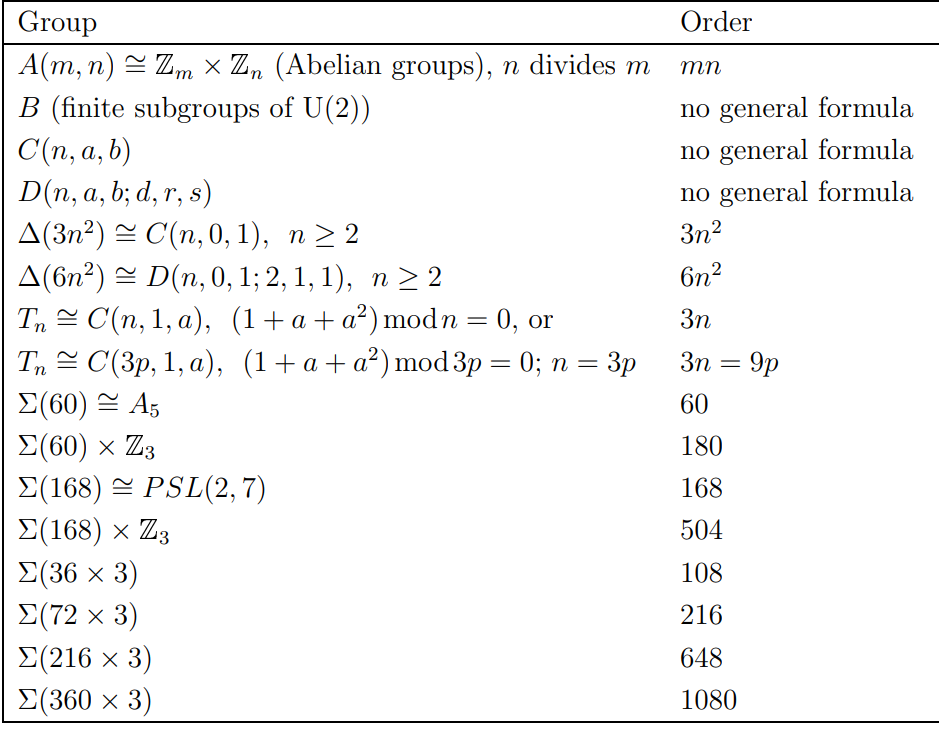
\includegraphics[scale=0.3]{img.png}
\end{figure}
Above is a table of all of the types of finite abelian subgroups that have been discovered. The only subgroup that I wish to discuss is the first one, as we are all familiar with the $\Z_m \times \Z_n$ groups\footnote{simple shorthand for $\Z/m\Z \times \Z/n\Z$}.
\begin{thm}
For all abelian subgroups A of $SU(3)$ is isomorphic to $\Z_m \times \Z_n$ such that $n|m$ and
\[ m = a' \]
we will denote $a'$ as the element $a \in A$ with the highest order.
\end{thm}
\begin{proof}
A is an abelian group of $3 \times 3$ matrices. Remember that for all $a \in A$ we need to make sure that $det(a) = 1$. Thus, if we are to create a basis for the group it would have to look like
\[
	\left[ \begin{matrix}
	a & 0 & 0\\
	0 & b & 0\\
	0 & 0 & a^{-1}b^{-1}
	\end{matrix} \right]
\]
such that $a,b \in U(1)$\\
This would then mean that $a^m = e$ where $e$ is the identity element. Suppose that for all $a \in A$ that $a^m \neq e$(m is not divisible by $|a|$). Let $g = gcd(|a|,m)$ and $g < |a|$. let $b$ be an element of $A$ such that $|b| = m$\\
This would then mean that $<a^g> \cap <b> = \{e\}$ for any $a,b \in A$, then
\[ |a^g \cdot b| = |a^g| \cdot |b| = \frac{|a|}{g} \cdot m > m\]
This leads to a contradiction to our earlier statement of $m = a'$.\\
From this, let $\mu = exp(2\pi i/m)$
\[
	\left[\begin{matrix}
	\mu^i & 0 & 0\\
	0 & \mu^j & 0\\
	0 & 0 & \mu^{-i-j}
	\end{matrix}\right]
\]
such that $0 \leq i,j \leq m-1$. We can then say that $A$ is a subgroup of:
\[
	\left\langle 
	\left[\begin{matrix}
	\mu & 0 & 0\\
	0 & 1 & 0\\
	0 & 0 & \mu^{-1}
	\end{matrix}\right],
	\left[\begin{matrix}
	1 & 0 & 0\\
	0 & \mu & 0\\
	0 & 0 & \mu^{-1}
	\end{matrix}\right] 	
	\right\rangle \cong \Z_m \times \Z_n
\]
Next we can treat m as a multiplicative sum of primes.
\[ m = p_1^{k_1} \times p_2^{k_2} \times ... \times p_i^{k_i} \]
\[ \Z_m = \Z_{p_1^{k_1}} \times \Z_{p_2^{k_2}} \times ... \times \Z_{p_i^{k_i}} \]
\[ \Z_m \times \Z_m = (\Z_{p_1^{k_1}} \times \Z_{p_1^{k_1}}) \times ... \times (\Z_{p_i^{k_i}} \times \Z_{p_i^{k_i}}) \]
\[ A \cong (\Z_{p_1^{r_1}} \times \Z_{p_1^{n_1}}) \times ... \times (\Z_{p_i^{r_i}} \times \Z_{p_i^{n_i}}) \cong \Z_r \times \Z_n \]
From out earlier proof by contradiction, we can then assume that r = m. Which shows that the isomorphism is true.\\
\end{proof}
\section{SU(3) and the Standard Model}
\subsection{Introduction to the Standard Model}
The standard model is the current best model for particles. Essentially, it is the best theory we have as of right now that explains why things exist and how the universe's building blocks interact with each other. The particles within the standard model can be labeled into four different categories. There are two main categories which then split off into two separate ones of themselves. \\\\
There are the elementary fermions; this is then split into quarks and leptons. There are six different types of quarks: up, down, charm, strange, top, and bottom. Then there are also six different leptons: the electrons, muons, tau, and neutrino versions for each of the three leptons. Quarks are what make up most of the atoms in our world. For example, protons contain two up quarks, one down quark, and neutrons containing two down quarks and one up quark.\\\\
Next are the elementary bosons, which are split into gauge bosons and scalar bosons. Gauge bosons are responsible for the different types of forces that we have observed in the universe consisting of photons(electromagnetic), W, Z(weak force), and gluons(strong force). Finally, the only scalar boson is the Higgs boson; this particle is essentially responsible for giving things mass in the world.\\\\
There are a lot more details that I have left out as the standard model is quite vast. However, what I do want to focus on are the relationship between the quarks, gluons, and SU(3)

\subsection{SU(3) and gluons}
According to the standard model, the connection between quarks is due to gluons. Each quark supposedly carries a color charge, either red, green or blue. In order for the gluons to connect these quarks, the gluon has to carry an anti-charge. So anti-red, ant-green or anti-blue. Logically, if you were to pair regular color charges and anti charges, there would be 9 different types of gluons. However, the standard model states that there are only eight.\\\\
Let r,b,g be red blue and green respectively, and $\bar{r}, \bar{b}, \bar{g}$ be the anti versions of the colors
\begin{align*}
	r &= \left[ \begin{matrix}
	1\\ 0\\ 0
	\end{matrix} \right]
	b = \left[ \begin{matrix}
	0\\ 1\\ 0
	\end{matrix} \right]
	g = \left[ \begin{matrix}
	0\\ 0\\ 1
	\end{matrix} \right] \\
	\bar{r} &= \left[ \begin{matrix}
	1 & 0 & 0
	\end{matrix} \right]
	\bar{b} = \left[ \begin{matrix}
	0 & 1 & 0
	\end{matrix} \right]
	\bar{g} = \left[ \begin{matrix}
	0 & 0 & 1
	\end{matrix} \right]
\end{align*}
With this representation we can say that this $3 \times 3$ matrix is the red and anti-blue connection
\[
	\left[ \begin{matrix}
	0 & 1 & 0\\
	0 & 0 & 0\\
	0 & 0 & 0
	\end{matrix} \right]
\]
This is because the 1 is in the top row, and the middle column, so $r$ and $\bar{b}$\\
If we apply this logic to the eight generators of $SU(3)$ we will get the eight different types of gluons.
\[
\lambda_1 = \left[ \begin{matrix}
	0 & 1 & 0\\
	1 & 0 & 0\\
	0 & 0 & 0
	\end{matrix} \right] = (r\bar{b} + b\bar{r})/\sqrt{2}
\]\[
\lambda_2 = \left[ \begin{matrix}
	0 & -i & 0\\
	i & 0 & 0\\
	0 & 0 & 0
	\end{matrix} \right] = -i(r\bar{b} - b\bar{r})/\sqrt{2}
\]\[
\lambda_3 = \left[ \begin{matrix}
	1 & 0 & 0\\
	0 & -1 & 0\\
	0 & 0 & 0
	\end{matrix} \right] = (r\bar{r} - b\bar{b})/\sqrt{2}
\]\[
\lambda_4 = \left[ \begin{matrix}
	0 & 0 & 1\\
	0 & 0 & 0\\
	1 & 0 & 0
	\end{matrix} \right] = (r\bar{g} + g\bar{r})/\sqrt{2}
\]\[
\lambda_5 = \left[ \begin{matrix}
	0 & 0 & -i\\
	0 & 0 & 0\\
	1 & 0 & 0
	\end{matrix} \right] = -i(r\bar{g} - g\bar{r})/\sqrt{2}
\]\[
\lambda_6 = \left[ \begin{matrix}
	0 & 0 & 0\\
	0 & 0 & 1\\
	0 & 1 & 0
	\end{matrix} \right] = (b\bar{g} + g\bar{b})/\sqrt{2}
\]\[
\lambda_7 = \left[ \begin{matrix}
	0 & 0 & 0\\
	0 & 0 & -i\\
	0 & i & 0
	\end{matrix} \right] = -i(b\bar{g} - g\bar{b})/\sqrt{2}
\]\[
\lambda_8 = \frac{1}{\sqrt{3}}\left[ \begin{matrix}
	1 & 0 & 0\\
	0 & 1 & 0\\
	0 & 0 & -2
	\end{matrix} \right] = (r\bar{r} + b\bar{b} - 2g\bar{g})/\sqrt{6}
\]
You can see that in this representation that the matrices all have to be Hermitian and traceless. This makes the group $SU(3)$ a perfect representation of the gluon colors. There eight "colors" are known as the color octet and they represent the eight states that a gluon can be in. Every single one of these states are linearly independent from each other, which means that it is impossible to recreate any of them by combining others together.

\section{Conclusion}
In conclusion, group theory is the study groups and is a subsection of abstract
algebra. It allows us to look at the symmetrical properties of mathematical
objects. Groups are sets with an attached binary operation, and in order for
that set to be considered as a group, it must satisfy four requirements called
the group axioms. In combination with Lie algebra, to create lie groups. We can take the Gell-Mann matrices to understand why there are only eight different types of gluon charge colors. Through this, we can see that even topics as abstract as group theory still has their uses and can be applied to things in the world we would normally overlook.
%----- ACKNOWLEDGEMENT SECTION -------------------------------------------------------------------
% Explain what the asterisk * does in the next line: 
\section*{Acknowledgements}
I would like to thank my Math 100 professor who first introduced me to LaTeX. I now use this program for almost all of my math assignments and am much better at this compared to writing it down.


%----- BIBLIOGRAPHY ------------------------------------------------------------------------------

% You will need to explain how to include the bibliography section as follows. Explain the environment and how to add new items.
% Including how \ref, \cite and \label should be included here.

% Reminder: you will need to explain how to include the Bibliography Section and then include your own Bibliography at the end of your own tutorial.

\begin{thebibliography}{1}

\bibitem{IEEEhowto:kopka}
H.~Kopka and P.~W. Daly, \emph{A Guide to {\LaTeX}}, 3rd~ed.\hskip 1em plus
  0.5em minus 0.4em\relax Harlow, England: Addison-Wesley, 1999.
\bibitem{ludlpatrick} Ludl, Patrick. Comments on the calssification of the finite subgroups of SU(3). {\it Journal of Algebra}. {\bf 114} (1988). pp. 115-259. 

\bibitem{ludlpatrick} Ludl, Patrick. Comments on the calssification of the finite subgroups of SU(3).(2011).

\bibitem{kiblermaurice} Kibler, Maurice. A Group-Theoretical Approach to the Periodic Table of Chemical Elements: Old and New Developments.

\bibitem{ludlpatrick} Kirillov, Alexander. Introduction to Lie Groups and Lie Algebras. 

\bibitem{ludlpatrick} Koerber, Christopher. Lie Algebra Tepresentation Theory-SU(3)-Representation in Physics.(2013) 

\bibitem{} “Why Are There Eight Gluons and Not Nine?” Why Are There Eight Gluons?, math.ucr.edu/home/baez/physics/ParticleAndNuclear/gluons.html. 
\end{thebibliography}



\end{document}
